\chapter*{Введение}                         % Заголовок
\addcontentsline{toc}{chapter}{Введение}    % Добавляем его в оглавление

\newcommand{\actuality}{}
\newcommand{\progress}{}
\newcommand{\aim}{{\textbf\aimTXT}}
\newcommand{\tasks}{\textbf{\tasksTXT}}
\newcommand{\novelty}{\textbf{\noveltyTXT}}
\newcommand{\influence}{\textbf{\influenceTXT}}
\newcommand{\methods}{\textbf{\methodsTXT}}
\newcommand{\defpositions}{\textbf{\defpositionsTXT}}
\newcommand{\reliability}{\textbf{\reliabilityTXT}}
\newcommand{\probation}{\textbf{\probationTXT}}
\newcommand{\contribution}{\textbf{\contributionTXT}}
\newcommand{\publications}{\textbf{\publicationsTXT}}


{\actuality} 

\textit{Квантовая электродинамика (КЭД)}, описывающая взаимодействие заряженных частиц и электромагнитного (ЭМ) поля, на данный момент является наиболее точной теорией, с точки зрения её экспериментальных проверок.
Однако ряд теоретических предсказаний нелинейной КЭД, основным из которых является образование электрон-позитронных пар из вакуума (эффект Заутера-Швингера)~\cite{Sauter31, Schwinger51} в сильном постоянном поле, впервые сделанных ещё в работах 30-х годов прошлого столетия, до сих пор не были подтверждены экспериментально.
С ожидаемым в ближайшие годы вступлением в строй лазерных установок нового поколения, таких как ELI~\cite{ELI}, Apollon~\cite{zou2015design}, SULF~\cite{SULF}, SEL~\cite{SEL}, XCELS~\cite{XCELS} и др., станет доступным экспериментальное исследование взаимодействия излучения с веществом в режиме экстремальной интенсивности, что открывает новые возможности для наблюдения эффектов \textit{сильнополевой} КЭД.
За определение, какое поле является сильным согласно КЭД, отвечают 4 Лоренц-инвариантных параметра: $a_0$, $\mathcal{F}$, $\mathcal{G}$, $\chi$.

Параметр $a_0$~---~классический параметр нелинейности~---~определяет безразмерную амплитуду внешнего ЭМ поля и существенность релятивистских эффектов
\begin{equation}
    a_0  = \frac{e}{mc}\sqrt{-A_\mu A^\mu} \equiv \frac{eE_0}{m c \omega},
\end{equation}
где $m$ и $e>0$~---~масса и модуль заряда электрона соответственно, $c$~---~скорость света, $A_\mu$~---~вектор-потенциал ЭМ поля, $E_0$ и $\omega$~---~характерная величина напряжённости и характерная частота изменения ЭМ поля соответственно.
При $a_0 > 1$ движение заряженных частиц становится релятивистским.
\fixme{аналогия с параметром Келдыша, ионизацией?}
\begin{equation}
  a_0 \approx 0.85 \sqrt{I[\SI{e18}{\watt/\centi\meter^2}]}\lambda[\si{\um}]
\end{equation}

Параметры $\mathcal{F}$, $\mathcal{G}$ фактически определяют взаимодействие ЭМ поля с \textit{вакуумом}
\begin{equation}
  \mathcal{F} = \frac{E^2 - B^2}{E_\mathrm{S}^2},
\end{equation}
\begin{equation}
  \mathcal{G} = \frac{\vb{E}\cdot\vb{B}}{E_\mathrm{S}^2},
\end{equation}
где $E_\mathrm{S} = m^2 c^3/e\hbar$~---~критическое поле КЭД или поле Заутера-Швингера~\cite{berestetskii1982quantum, Baier98}, $\hbar$~---~постоянная Планка.
Эффект образования электрон-позитронных пар из вакуума является экспоненциально подавленным при $|\mathcal{F}|\lesssim 1$, что объясняет трудность его экспериментального наблюдения.
При этом, например, двулучепреломление вакуума~\cite{dirac1934discussion, serber1935linear, uehling1935polarization, heisenberg1936folgerungen}, также являющееся одним из наиболее ранних предсказаний КЭД, и которое определяется величинами $\mathcal{F}$ и $\mathcal{G}$, подтверждается в экспериментах в области $|\mathcal{F}|\ll 1$ как косвенно~\cite{bennett2006final, hanneke2008new}, так и напрямую~\cite{atlas2017evidence}.
Отметим, что поля лазерных импульсов и пучков заряженных частиц (см. ниже) являются скрещенными, поэтому в таких конфигурациях значения параметров $\mathcal{F}$ и $\mathcal{G}$ близки к нулю.
Далее в работе всегда будет предполагаться выполнение условия $\mathcal{F} = \mathcal{G} = 0$.

Наконец, параметр $\chi$ определяет существенность чисто квантовых эффектов при взаимодействии ЭМ поля с частицами
\begin{equation}
    \chi = \frac{e\hbar\sqrt{-\left( F_{\mu\nu}p^\nu \right)^2}}{m^3c^4} = \frac{1}{E_\mathrm{S} mc} \sqrt{{\left( \frac{\varepsilon}{c}\vb{E} + \vb{p}\times\vb{B} \right)}^2 - {\left(\vb{p}\vb{E} \right)}^2} ,
\end{equation}
где $F_{\mu\nu}=\partial_\mu A_\nu - \partial_\nu A_\mu$~---~тензор ЭМ поля, $\varepsilon$ и $\vb{p}$~---~энергия и импульс частицы.
Данное выражение записывается для фотонов аналогичным образом с учётом того, что $\varepsilon=\hbar\omega$, $p^\nu=\hbar k^\nu$.
Здесь необходимо указать на важную дистинкцию между квантовым описанием ЭМ поля как совокупности фотонов и классическим описанием через напряжённости поля.
При больших числах заполнения квантовое описание совпадает с классическим, таким образом относительно сильные внешние поля описываются классически, а единичные фотоны, образующиеся в результате КЭД процессов, с помощью собственно квантового подхода.
Более того взаимодействие электронов (и позитронов) с сильным классическим полем ($a_0 > 1$) должно учитываться непертурбативно, т.е. во всех порядках теории возмущений, что делается с помощью представления Фарри~\cite{furry1951bound} и использования Волковских функций для описания состояния электронов~\cite{wolkow1935klasse} (более подробно данная особенность описана, например, в обзоре~\cite{fedotov2022QED}).
Классическое внешнее поле также зачастую существенно отличается от фотонов, образующихся при движении частиц в этом внешнем поле, со спектральной точки зрения.
Так, экстремально сильные ЭМ поля доступны сейчас преимущественно в оптическом диапазоне $\hbar\omega_L\sim\SI{1}{\electronvolt}$, тогда как характерная частота излучения частиц в таком поле, которую можно оценить по синхротронным формулам как $\hbar\omega\sim\gamma^3\hbar\omega_L$, обычно лежит в области рентгена или даже гамма-диапазоне.

В режиме $\chi > 1$ становятся вероятными квантовые процессы приводящие к образованию электрон-позитронных пар.
К ним относятся, например, процесс Брейта-Уиллера~\cite{breit1934collision}, в котором жёсткий фотон <<распадается>> на электрон-позитронную пару, и процесс Бете-Гайтлера (\textit{трайдент}-процесс)~\cite{bethe1934stopping}, в котором электрон или позитрон излучает виртуальный фотон, который в последствии распадается на электрон-позитронную пару (см. Рис.~\ref{fig:intro/QED}). 
\begin{figure}[ht]
  \begin{minipage}[b][][b]{0.49\linewidth}\centering
      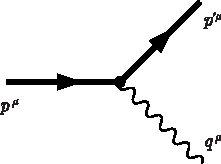
\includegraphics[width=0.5\linewidth]{intro-Compton-NL} 
  \end{minipage}
  \hfill
  \begin{minipage}[b][][b]{0.49\linewidth}\centering
      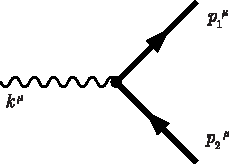
\includegraphics[width=0.5\linewidth]{intro-Breit-Wheeler-NL}
  \end{minipage}
  \caption{\fixme{Элементарные КЭД процессы во внешнем поле. (Добавить трайдент)}}
  \label{fig:intro/QED}
\end{figure}
Эти процессы являются экспоненциально подавленными при $\chi \lesssim 1$ и во многом аналогичны процессу образования электрон-позитронных пар по механизму Заутера-Швингера.
В силу того, что параметр $\chi$, помимо напряжённости ЭМ поля, определяется энергией частицы, ожидается, что экспериментальное наблюдение описанных таких процессов может быть возможным, например, на упомянутых выше лазерных установках нового поколения.
Однако, даже в режиме $\chi \lesssim 1$, когда образование электрон-позитронных пар подавлено, взаимодействие заряженных частиц с ЭМ полем может существенно изменяться за счёт реакции излучения.
Сам факт того, что заряженные частицы испытывают силу отдачи при излучении известен уже более века и изначально был описан в рамках классической электродинамики, однако привёл к противоречивости понятия об электроне как о точечном объекте и обозначил границу применимости классической ЭД, которую можно определить условием ${E_\mathrm{cl} = m^2 c^4 / e^3 = E_\mathrm{S} / \alpha}$.
Поле такой напряжённости создаёт электрон на расстоянии своего классического радиуса $r_e = e^2 / m c^2$.
Отметим, что оно в ${1/\alpha \approx 137}$ раз больше критического поля КЭД, поэтому квантовые эффекты появляются <<раньше>>, чем становится противоречивой классическая ЭД. 
Квантовая электродинамика описывает излучение фотонов электронами непротиворечивым образом и совпадает с результатами классической ЭД в пределе ${\chi\ll1}$.
Отдельный интерес, однако, представляет модификация спектра излучения и существенный эффект отдачи в режиме $\chi \gtrsim 1$, который практически не исследован экспериментально.
До недавнего времени существовал лишь единственный пример из 1990-х годов, а именно эксперимент E-144 на ускорителе SLAC \fixme{($a_0 \ll 1$, $\chi \ll 1$)}, где электронный пучок с энергией $\SI{46.6}{\giga\electronvolt}$ взаимодействовал с лазерным импульсом мощностью ${I\sim\SI{e18}{\watt/\centi\meter^2}}$, производя фотоны высокой энергии, которые, в свою очередь, превращались в электрон-позитронные пары в электромагнитном поле лазерного импульса~\cite{bula1996observation, burke1997positron}.
Недавно концептуально схожие  эксперименты были проведёны на установке Astra Gemini, где один лазерный импульс использовался для ускорения электронов, а второй~---~для рассеяния на ускоренных электронах~\cite{Poder17, Cole17} \fixme{($a_0 \sim 1$, $\chi \lesssim 1$)}.
Важно отметить, что несмотря на неоспоримую ценность этих экспериментов, их результаты содержат определённый уровень погрешности, который не позволяет с уверенностью заявлять о точности предсказаний КЭД.
Благодаря развитию технологий как лазерных установок, так и ускорителей, в ближайшем будущем ожидаются новые эксперименты по физике сильных полей, в частности прямой наследник эксперимента E-144~---~эксперимент E-320, на котором ожидается достижение существенно квантового режима взаимодействия~\cite{meuren2019probing} \fixme{($a_0 > 1$, $\chi > 1$)}.
Тем временем стремительно растёт число теоретических исследований, предсказывающих новые эффекты, вызванные влиянием реакции излучения на коллективные процессы.
Эти эффекты крайне различны и включают в себя, например, изменение механизмов ускорения частиц~\cite{Tamburini10, Tamburini12, kostyukov2012radiative, Capdessus12, Capdessus15, Nerush15, Gelfer18a, Gelfer18b, gelfer2021ions, golovanov2021radiation},
\fixme{радиационный захват частиц~\cite{Gonoskov14, Ji14b}}
крайне эффективное поглощение лазерного излучения~\cite{grismayer2016laser},
подавление релятивистской прозрачности~\cite{Zhang15, serebryakov2022opacity},
обратный эффект Фарадея~\cite{Liseykina16,liseykina2021IFE},
поляризацию частиц~\cite{DelSorbo2017Spin,DelSorbo2018spin,Chen2019spin,Seipt2019spin,Wu2019spin,li2019ultrarelativistic,Li2020spin,Wan2020spin,gong2021retrieving} и много других.

В режиме $\chi\gtrsim 1$ предполагается, что поведение вещества в экстремальных ЭМ полях в большом числе конфигураций во многом определяется развитием \textit{квантово-электродинамических каскадов}~\cite{nerush2007radiation,Bell2008,Nerush11a,Ridgers12,narozhny2015quantum,Kostyukov2016,grismayer2017seeded,jirka2017qed,luo2018qed,Yuan2018,del2018ion,Lu2018,Luo2018,efimenko2019laser}.
Суть КЭД каскада состоит в излучении жёстких фотонов ультрарелятивистскими частицами в результате нелинейного комптоновского рассеяния и последующий <<распад>> первых на электрон-позитронные пары в результате процесса Брейта-Уиллера\footnote{ Как было отмечено выше образование электрон-позитронной пары также возможно напрямую из электрона во внешнем в результате процесса Бете-Гайтлера}. 
Вторичные частицы также становятся вовлечены в образовании следующего поколения пар, что приводит к лавинообразному росту числа частиц.
Развитие таких каскадов качественно похоже на другой физический процесс~---~лавинообразную ионизацию при пробое в газе~\cite{raizer1997gas}.
Активное исследование микроволнового пробоя в газах выявило достаточно сложную динамику данного процесса, сопровождаемую образованием плазмы и генерацией волн пробоя~\cite{bollen1983high,semenov1982breakdown}.
Аналогия между рождением пар в вакууме и ионизацией газа, или между \textit{пробоем вакуума} в результате развития КЭД каскада и газового пробоя имеет глубокое физическое обоснование~\cite{dunne2012,narozhny2015quantum,efimenko2018extreme}.
Считается, что процессы развития КЭД каскадов играют немаловажную роль в различных астрофизических феноменах, таких как космические ливни~\cite{bhabha1937passage}, гамма-вспышки~\cite{meszaros2006gamma}, процессах в магнитосфере пульсаров~\cite{sturrock1971model,ruderman1975theory,daugherty1982electromagnetic, philippov2015ab} и др. 
Разнообразие и сложность образующихся в результате развития КЭД каскада структуры электрон-позитронной плазмы объясняет их активное исследование, далёкое от завершения.

Лабораторное моделирование астрофизических процессов (\textit{лабораторная астрофизика}) за счёт использования экстремально интенсивных лазеров является нетривиальной задачей с точки зрения постановки и интерпретации результатов эксперимента.
Во многом это связано с тем, что ключевую роль в астрофизических процессах играет взаимодействие потоков частиц друг с другом, поэтому для лабораторного моделирования таких процессов необходимо сначала создать такие потоки частиц с помощью лазера.
В этой связи, также исследуются альтернативные возможности, например, использование коллайдеров, являющихся основным инструментом исследований в области физики элементарных частиц, и которые основаны на лобовом столкновении пучков заряженных частиц высокой энергии.
В настоящее время существует несколько проектов, нацеленных на строительство высоко-энергетических лептонных коллайдеров с рекордными параметрами, таких как ILC~\cite{ILC} и CLIC~\cite{CLIC}.
Относительно недавно плазменное ускорение стало рассматриваться в качестве привлекательного альтернативного метода создания линейных коллайдеров с большим ускоряющим градиентом~\cite{schroeder2010physics}.
В области взаимодействия на таких коллайдерах могут генерироваться сильные ЭМ поля, благодаря чему возможно проявление таких эффектов, как \textit{разрушение} пучков (\textit{disruption})~\cite{hollebeek1981disruption,yokoya1992beam,chen1988disruption}, \textit{пучковое излучение} (\textit{beamstrahlung})~\cite{noble1987beamstrahlung,blankenbecler1987quantum,bell1995quantum}, образование вторичных электрон-позитронных пар~\cite{chen1989coherent,esberg2014strong}, и даже эффектов \textit{непертурбативной} сильнополевой КЭД~\cite{yakimenko2019prospect,tamburini2020efficient}.
Так как достижение всё больших интенсивностей излучения на лазерных установках предъявляет всё более жёсткие требования к контрасту, стабильности, качеству пучка, пока не достигнутые на практике~\cite{danson2019petawatt}, сильноточные высокоэнергетические коллайдеры, отличающиеся высоким качеством и стабильностью пучка, могут стать привлекательной <<безлазерной>> альтернативой для экспериментов в области физики сильного поля.
Наиболее активно в таком контексте обсуждается проект FACET-II, посвященный изучению плазменного ускорения~\cite{FACET, yakimenko2019prospect, del2019bright, meuren2019probing}.

Таким образом, исследование физики сильных полей представляет как фундаментальный интерес, так и практическое значение.

% \ifsynopsis
% Этот абзац появляется только в~автореферате.
% Для формирования блоков, которые будут обрабатываться только в~автореферате,
% заведена проверка условия \verb!\!\verb!ifsynopsis!.
% Значение условия задаётся в~основном файле документа (\verb!synopsis.tex! для
% автореферата).
% \else
% Этот абзац появляется только в~диссертации.
% Через проверку условия \verb!\!\verb!ifsynopsis!, задаваемого в~основном файле
% документа (\verb!dissertation.tex! для диссертации), можно сделать новую
% команду, обеспечивающую появление цитаты в~диссертации, но~не~в~автореферате.
% \fi

\vspace{0.25cm}
{\aim} данной работы является исследование влияния реакции излучения и образования электрон-позитронных пар на процессы, происходящие в экстремально сильных электромагнитных полях в различных конфигурациях, в частности при взаимодействии лазерного излучения с твердотельной мишенью, столкновении сильноточных пучков ультрарелятивистских частиц друг с другом и с плазменной мишенью.

Для~достижения поставленной цели были поставлены следующие {\tasks}:
\begin{enumerate}[beginpenalty=10000] % https://tex.stackexchange.com/a/476052/104425
  \item Разработать теорию движения отдельных заряженных частиц в сильных полях в режиме экстремальных радиационных потерь. Определить общие свойства движения частиц согласно разработанной модели. Применить теорию в различных конфигурациях электромагнитного поля. Определить область применимости модели, в частности путём сравнения полученных результатов с результатами, полученными численными методами.
  \item Исследовать взаимодействие лазерного импульса экстремальной интенсивности с твердотельной мишенью с помощью численного моделирования. Определить особенности и механизм развития квантово-электро\-динамического каскада при таком взаимодействии.
  \item Разработать аналитическую модель развития квантово-электро\-динамического каскада в поле плоской волны. Определить точность разработанной модели путём сравнения с результатами численного моделирования.
  \item Исследовать влияние реакции излучения на процесс фокусировки пучков ультрарелятивистских частиц при их лобовом столкновении. Разработать модель для вычисления параметра разрушения с учётом реакции излучения. Сравнить полученные аналитические результаты с результатами численного моделирования.
  \item Исследовать процесс генерации гамма-излучения при взаимодействии сильноточного пучка ультрарелятивистских электронов с плазменной мишенью с помощью численного моделирования. Разработать модели для вычисления эффективности конверсии энергии пучка в энергию гамма-излучения. Определить параметры пучка на установке FACET-II, оптимальные с точки зрения генерации гамма-излучения.
  \item Разработать численную схему решения уравнений Максвелла на сетке с подавленной черенковской неустойчивостью.
\end{enumerate}

\vspace{0.25cm}
{\novelty}
\begin{enumerate}[beginpenalty=10000] % https://tex.stackexchange.com/a/476052/104425
  \item Разработана асимптотическая теория движения заряженных частиц в режиме экстремальных радиационных потерь. Определены общие свойства движения частиц в таком режиме, существенно отличающиеся от таковых в режиме слабой реакции излучения. Продемонстрирован новый метод получения приближённого решения уравнений движения в различных конфигурациях.
  \item Обнаружен и качественно описан эффект развития самоподдерживающегося квантово-электродинамического каскада в поле, приближенном к полю плоской волны. Разработана аналитическая модель, описывающая развитие такого каскада.
  \item Разработана модель для вычисления параметра разрушения при лобовом столкновении сильноточных пучков ультрарелятивистских частиц с учётом реакции излучения. Достоверность модели подтверждена полноразмерным численным трёхмерным моделированием
  \item С помощью полноразмерного трёхмерного численного моделирования продемонстрирована схема эффективной генерации гамма-излучения при взаимодействии сильноточного пучка ультрарелятивистских электронов с протяжённой плазменной мишенью. Разработана аналитическая модель для вычисления эффективности конверсии энергии пучка в энергию гамма-излучения. Найдены параметры пучка для установки FACET-II, оптимальные с точки зрения генерации гамма-излучения.
  \item Разработана и реализована в коде QUILL альтернативная схема для численного решения уравнений Максвелла на регулярной сетке, отличающаяся существенно подавленной численной черенковской неустойчивостью, и подходящей для моделирования пучков ультрарелятивистских частиц.
\end{enumerate}

\vspace{0.25cm}
{\influence}
\begin{enumerate}[beginpenalty=10000]
  \item Разработанная теория движения частиц в условиях экстремальных радиационных потерь может быть использована в качестве дополнительного аналитического инструмента для определения динамики частиц в различных конфигурациях электромагнитного поля.
  \item Проведённое численное моделирование процесса взаимодействия экстремально интенсивного слабо-сфокусированного лазерного излучения с тонкой твердотельной мишенью расширяет класс конфигураций электромагнитного поля, в которых возможно наблюдение самоподдерживающегося квантово-электродинамического каскада.
  \item Разработанная аналитическая модель развития квантово-электро\-динамического каскада в плоской волне, учитывающая пространственную, а не только временную, динамику частиц может быть адаптирована для исследования развития квантово-электродинамических каскадов в других конфигурациях, например, при взаимодействии лазерного излучения с различными мишенями, пучками частиц, взаимодействие пучков друг с другом. 
  \item Проведённое численное моделирование и разработанная аналитическая модель усиления фокусировки сильноточных пучков при их столкновении за счёт реакции излучения может быть использована для уточнения требуемых параметров пучков при проведении экспериментов на коллайдерах и ускорителях нового поколения, таких как CLIC, ILC, FACET-II.
  \item Проведённое численное моделирование взаимодействия сильноточного пучка ультрарелятивистских частиц с протяжённой плазменной мишенью может быть использовано для планирования экспериментов на коллайдерах и ускорителях нового поколения по генерации яркого гамма-излучения. 
  \item Разработанная схема для численного решения уравнений Максвелла на сетке с подавленной черенковской неустойчивостью может быть реализована в PIC-кодах для существенного увеличения достоверности результатов моделирования процессов с участием пучков ультрарелятивистских частиц.
\end{enumerate}

% {\methods} \ldots

\vspace{0.25cm}
{\defpositions}
\begin{enumerate}[beginpenalty=10000] % https://tex.stackexchange.com/a/476052/104425
  \item Первое положение
  \item Второе положение
  \item Третье положение
  \item Четвертое положение
\end{enumerate}
% В папке Documents можно ознакомиться с решением совета из Томского~ГУ
% (в~файле \verb+Def_positions.pdf+), где обоснованно даются рекомендации
% по~формулировкам защищаемых положений.

\vspace{0.25cm}
{\reliability} полученных результатов обеспечивается использованием надёжных физических моделей и применением теоретических методов, имеющих строгое математическое обоснование, таких как теория возмущений,
разложение в ряд по малому параметру, усреднение по <<быстрому>> времени и др. 
Результаты сопоставлялась с результатами, полученными с помощью различных численных методов, в частности полномасштабного трехмерного численного моделирования, основанного на базовых физических принципах, а также с результатами, полученными ранее другими авторами.

\vspace{0.25cm}
{\probation}
Основные результаты диссертации докладывались на семинарах ИПФ РАН, а также на следующих конференциях, в том числе лично:
\begin{enumerate}
    \item XXII Научная конференция по радиофизике, Нижний Новгород, Россия, 2018;
    \item XXVIII Научная школа «Нелинейные волны 2018», Нижний Новгород, Россия;
    \item XXIII Научная конференция по радиофизике, Нижний Новгород, Россия, 2019;
    \item VII International Conference “Frontiers of Nonlinear Physics”, Nizhny Novgorod, Russia, 2019;
    \item XIX Научная школа «Нелинейные волны 2020», Нижний Новгород, Россия, 2020;
    \item IV International Conference <<UltrafastLight-2020>>, Moscow, Russia, 2020;
    \item ELI-NP Autumn School, Magurele, Romania, 2020;
    \item 20 международная конференция и молодёжная школа «Математическое моделирование и суперкомпьютерные технологии», Нижний Новгород, Россия, 2020;
    \item 63-я Всероссийская научная конференция МФТИ, Москва, Россия, 2020;
    \item The 2nd China-Russia Frontier Seminar on Ultra Intense Laser Technology and Intense Field Physics, Nizhny Novgorod, Russia, 2020;
    \item EPS 47th Conference on Plasma Physics, Sitges, Spain, 2021;
    \item 29th annual International Laser Physics Workshop, Lyon, France, 2021;
    \item V International Conference <<UltrafastLight-2021>>, Moscow, Russia, 2021;
    \item 18th International Workshop Complex Systems of Charged Particles and Their Interactions with Electromagnetic Radiation, Moscow, Russia, 2022;
    \item 30th annual International Laser Physics Workshop, Lyon, France, 2022.
\end{enumerate}

\vspace{0.25cm}
{\contribution} Основные положения, выносимые на защиту, отражают личный вклад автора в опубликованные работы.
Подготовка к публикации полученных результатов проводилась совместно с соавторами, причем вклад диссертанта был определяющим.
Все представленные в диссертации результаты получены лично автором.

\vspace{0.25cm}
{\publications} Основные результаты по теме диссертации изложены в~\total{citeauthor}~печатных изданиях, \total{citeauthorscopuswos} из которых изданы в~периодических научных журналах, индексируемых Web of~Science и Scopus~\autocite{artemenko2016formation, samsonov2018asymptotic, samsonov2019laser, samsonov2020superluminal, samsonov2021hydrodynamical, samsonov2021effect, samsonov2021beamstrahlung, filipovic2021effect, samsonov2022simulation, samsonov2022high}, \total{citeauthorconf} "--- в~тезисах докладов~\cite{samsonov2018NW, samsonov2019FNP, samsonov2020NW, samsonov2020UFL, samsonov2020Math, samsonov2021EPS, samsonov2021UFL, samsonov2021LPHYS, samsonov2022CSCPIER, samsonov2022LPHYS}.

% \begin{refsection}[bl-author]
% \end{refsection}

\begin{comment}
\ifnumequal{\value{bibliosel}}{0}
{%%% Встроенная реализация с загрузкой файла через движок bibtex8. (При желании, внутри можно использовать обычные ссылки, наподобие `\cite{vakbib1,vakbib2}`).
    {\publications} Основные результаты по теме диссертации изложены
    в~XX~печатных изданиях,
    X из которых изданы в журналах, рекомендованных ВАК,
    X "--- в тезисах докладов.
}%
{%%% Реализация пакетом biblatex через движок biber
    \begin{refsection}[bl-author]
        % Это refsection=1.
        % Процитированные здесь работы:
        %  * подсчитываются, для автоматического составления фразы "Основные результаты ..."
        %  * попадают в авторскую библиографию, при usefootcite==0 и стиле `\insertbiblioauthor` или `\insertbiblioauthorgrouped`
        %  * нумеруются там в зависимости от порядка команд `\printbibliography` в этом разделе.
        %  * при использовании `\insertbiblioauthorgrouped`, порядок команд `\printbibliography` в нём должен быть тем же (см. biblio/biblatex.tex)
        %
        % Невидимый библиографический список для подсчёта количества публикаций:
        % \printbibliography[heading=nobibheading, section=1, env=countauthorvak,          keyword=biblioauthorvak]%
        % \printbibliography[heading=nobibheading, section=1, env=countauthorwos,          keyword=biblioauthorwos]%
        % \printbibliography[heading=nobibheading, section=1, env=countauthorscopus,       keyword=biblioauthorscopus]%
        % \printbibliography[heading=nobibheading, section=1, env=countauthorconf,         keyword=biblioauthorconf]%
        % \printbibliography[heading=nobibheading, section=1, env=countauthorother,        keyword=biblioauthorother]%
        % \printbibliography[heading=nobibheading, section=1, env=countauthor,             keyword=biblioauthor]%
        % \printbibliography[heading=nobibheading, section=1, env=countauthorvakscopuswos, filter=vakscopuswos]%
        % \printbibliography[heading=nobibheading, section=1, env=countauthorscopuswos,    filter=scopuswos]%
        % %
        % \nocite{*}%
        %
        % {\publications} Основные результаты по теме диссертации изложены в~\arabic{citeauthor}~печатных изданиях,
        % \arabic{citeauthorvak} из которых изданы в журналах, рекомендованных ВАК\sloppy%
        % \ifnum \value{citeauthorscopuswos}>0%
        %     , \arabic{citeauthorscopuswos} "--- в~периодических научных журналах, индексируемых Web of~Science и Scopus\sloppy%
        % \fi%
        % \ifnum \value{citeauthorconf}>0%
        %     , \arabic{citeauthorconf} "--- в~тезисах докладов.
        % \else%
        %     .
        % \fi%

        {\publications} Основные результаты по теме диссертации изложены в~\total{citeauthor}~печатных изданиях, \total{citeauthorscopuswos} из которых изданы в~периодических научных журналах, индексируемых Web of~Science и Scopus~\cite{artemenko2016formation, samsonov2018asymptotic, samsonov2019laser, samsonov2021hydrodynamical, samsonov2021beamstrahlung, filipovic2021effect, samsonov2021effect, samsonov2022simulation, samsonov2022high}, \total{citeauthorconf} "--- в~тезисах докладов~\cite{samsonov2018NW, samsonov2019FNP, samsonov2020NW, samsonov2022LPHYS}.

        % \ifnum \value{citeregistered}=1%
        %     \ifnum \value{citeauthorpatent}=1%
        %         Зарегистрирован \arabic{citeauthorpatent} патент.
        %     \fi%
        %     \ifnum \value{citeauthorprogram}=1%
        %         Зарегистрирована \arabic{citeauthorprogram} программа для ЭВМ.
        %     \fi%
        % \fi%
        % \ifnum \value{citeregistered}>1%
        %     Зарегистрированы\ %
        %     \ifnum \value{citeauthorpatent}>0%
        %     \formbytotal{citeauthorpatent}{патент}{}{а}{}\sloppy%
        %     \ifnum \value{citeauthorprogram}=0 . \else \ и~\fi%
        %     \fi%
        %     \ifnum \value{citeauthorprogram}>0%
        %     \formbytotal{citeauthorprogram}{программ}{а}{ы}{} для ЭВМ.
        %     \fi%
        % \fi%
        % К публикациям, в которых излагаются основные научные результаты диссертации на соискание учёной
        % степени, в рецензируемых изданиях приравниваются патенты на изобретения, патенты (свидетельства) на
        % полезную модель, патенты на промышленный образец, патенты на селекционные достижения, свидетельства
        % на программу для электронных вычислительных машин, базу данных, топологию интегральных микросхем,
        % зарегистрированные в установленном порядке.(в ред. Постановления Правительства РФ от 21.04.2016 N 335)
    \end{refsection}%
    \begin{refsection}[bl-author]
        % Это refsection=2.
        % Процитированные здесь работы:
        %  * попадают в авторскую библиографию, при usefootcite==0 и стиле `\insertbiblioauthorimportant`.
        %  * ни на что не влияют в противном случае
        % \nocite{vakbib2}%vak
        % \nocite{patbib1}%patent
        % \nocite{progbib1}%program
        % \nocite{bib1}%other
        % \nocite{confbib1}%conf
        % \nocite{samsonov2020superluminal}
    \end{refsection}%
        %
        % Всё, что вне этих двух refsection, это refsection=0,
        %  * для диссертации - это нормальные ссылки, попадающие в обычную библиографию
        %  * для автореферата:
        %     * при usefootcite==0, ссылка корректно сработает только для источника из `external.bib`. Для своих работ --- напечатает "[0]" (и даже Warning не вылезет).
        %     * при usefootcite==1, ссылка сработает нормально. В авторской библиографии будут только процитированные в refsection=0 работы.
}
\end{comment}

% При использовании пакета \verb!biblatex! будут подсчитаны все работы, добавленные
% в файл \verb!biblio/author.bib!. Для правильного подсчёта работ в~различных
% системах цитирования требуется использовать поля:
% \begin{itemize}
%         \item \texttt{authorvak} если публикация индексирована ВАК,
%         \item \texttt{authorscopus} если публикация индексирована Scopus,
%         \item \texttt{authorwos} если публикация индексирована Web of Science,
%         \item \texttt{authorconf} для докладов конференций,
%         \item \texttt{authorpatent} для патентов,
%         \item \texttt{authorprogram} для зарегистрированных программ для ЭВМ,
%         \item \texttt{authorother} для других публикаций.
% \end{itemize}
% Для подсчёта используются счётчики:
% \begin{itemize}
%         \item \texttt{citeauthorvak} для работ, индексируемых ВАК,
%         \item \texttt{citeauthorscopus} для работ, индексируемых Scopus,
%         \item \texttt{citeauthorwos} для работ, индексируемых Web of Science,
%         \item \texttt{citeauthorvakscopuswos} для работ, индексируемых одной из трёх баз,
%         \item \texttt{citeauthorscopuswos} для работ, индексируемых Scopus или Web of~Science,
%         \item \texttt{citeauthorconf} для докладов на конференциях,
%         \item \texttt{citeauthorother} для остальных работ,
%         \item \texttt{citeauthorpatent} для патентов,
%         \item \texttt{citeauthorprogram} для зарегистрированных программ для ЭВМ,
%         \item \texttt{citeauthor} для суммарного количества работ.
% \end{itemize}
% Счётчик \texttt{citeexternal} используется для подсчёта процитированных публикаций;
% \texttt{citeregistered} "--- для подсчёта суммарного количества патентов и программ для ЭВМ.

% Для добавления в список публикаций автора работ, которые не были процитированы в
% автореферате, требуется их~перечислить с использованием команды \verb!\nocite! в
% \verb!Synopsis/content.tex!.
 % Характеристика работы по структуре во введении и в автореферате не отличается (ГОСТ Р 7.0.11, пункты 5.3.1 и 9.2.1), потому её загружаем из одного и того же внешнего файла, предварительно задав форму выделения некоторым параметрам

\textbf{Объем и структура работы.} Диссертация состоит из~введения,
\formbytotal{totalchapter}{глав}{ы}{}{},
заключения.
%% на случай ошибок оставляю исходный кусок на месте, закомментированным
%Полный объём диссертации составляет  \ref*{TotPages}~страницу
%с~\totalfigures{}~рисунками и~\totaltables{}~таблицами. Список литературы
%содержит \total{citenum}~наименований.
%
Полный объём диссертации составляет
\formbytotal{TotPages}{страниц}{у}{ы}{}, включая
\formbytotal{totalcount@figure}{рисун}{ок}{ка}{ков} и
\formbytotal{totalcount@table}{таблиц}{у}{ы}{}.
Список литературы содержит
\formbytotal{citenum}{наименован}{ие}{ия}{ий}.
